%!TEX root = ../Thesis.tex
\chapter{Miscellaneous} \label{app:misc}

\section{Implicit Euler algorithm} \label{app:implicit_euler}
All new values $(x,y,p_x,p_y)_{i+1}$ refer to the same unknown values in the same time step $(x,y,p_x,p_y)_{i+1}$.
\begin{align}
    X_{i+1} &= X_i + (P_{X,i+1} + Y_{i+1})h, \\[0.2cm]
    Y_{i+1} &= Y_i + (P_{Y,i+1} - X_{i+1})h , \\[0.2cm]
    P_{X,i+1} &= P_{X,i} + \left(P_{Y,i+1} - \dfrac{(1-k)(k+X_{i+1})}{((k+X_{i+1})^2+Y_{i+1}^2)^{3/2}} + \dfrac{k(X_{i+1}-1+k)}{((X_{i+1}-1+k)^2+Y_{i+1}^2)^{3/2}}\right)h, \\[0.2cm]
    P_{Y,i+1} &= P_{Y,i} + \left(-P_{X,i+1} - \dfrac{(1-k)Y_{i+1}}{((k+X_{i+1})^2+Y_{i+1}^2)^{3/2}} - \dfrac{k Y_{i+1}}{((X_{i+1}-1+k)^2+Y_{i+1}^2)^{3/2}}\right)h.
\end{align}

\section{Restricted Three-Body Problem Symplectic Euler Derivations (Mathematica)} \label{app:r3b-symplectic-euler}
\begin{figure}[h!]
\centering 
\includegraphics[scale=0.8]{appendices/Miscellaneous/symplectic_euler_derivation.pdf}
\end{figure}

\section{Restricted Three-Body Problem Störmer-Verlet Derivations (Mathematica)} \label{app:r3b-verlet}
\begin{figure}[h!]
\centering 
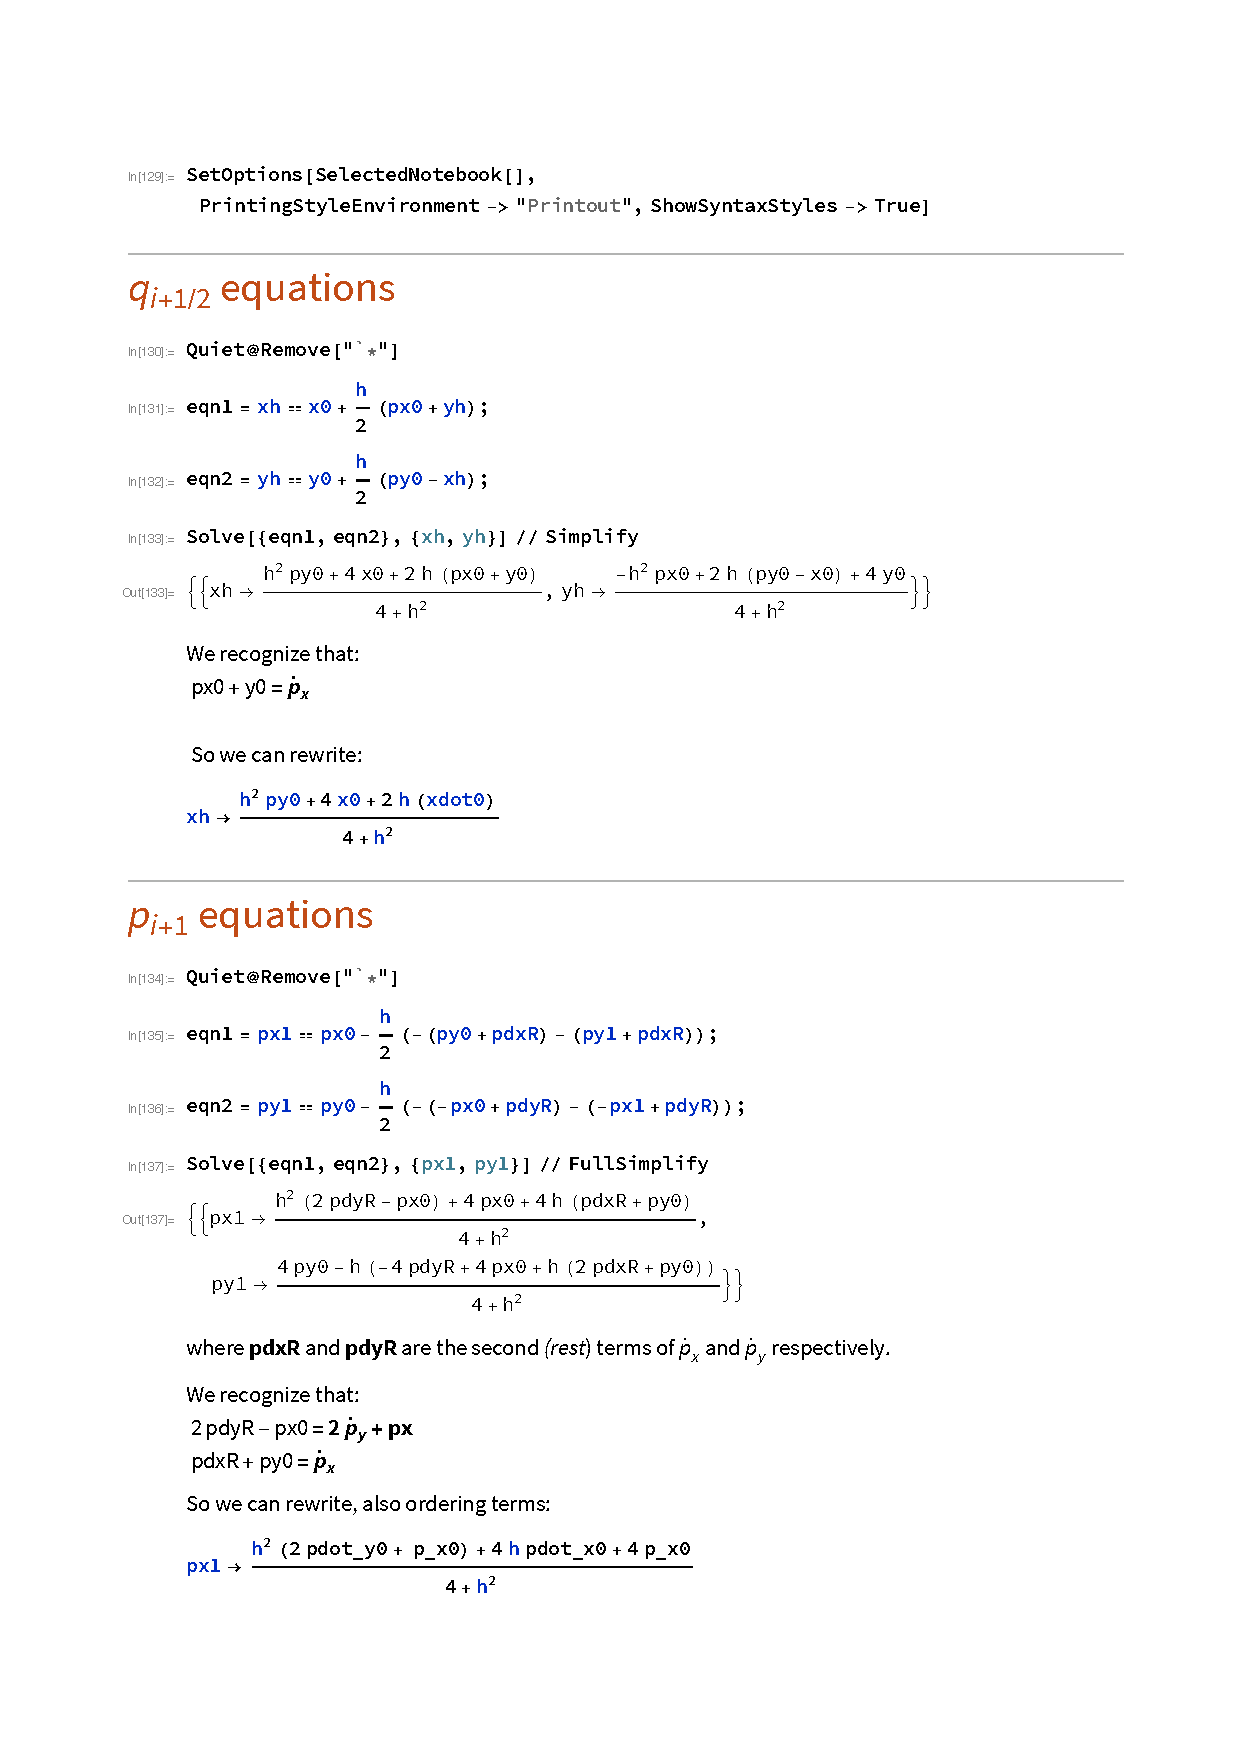
\includegraphics[scale=0.60]{appendices/Miscellaneous/R3B_Verlet_derivations.pdf}
\end{figure}


\clearpage

\section{Medium and Short Hohmann orbits} \label{app:more_hohmann}
\begin{adjustwidth*}{0cm}{-0.4cm}
\begin{lstlisting}[language=Python,caption=Medium duration Hohmann]
# --------------------------------------------------------------------------
duration = 3/unit_time
pos      = -2.272183066647597
ang      = -0.075821466029764
burn     = 3.135519748743719/unit_vel
x0       = -0.023110975767437
y0       = -0.012972499765730
px0      = 8.032228991913522
py0      = -7.100537706154897
# --------------------------------------------------------------------------
# dV(earth-escape) = 3.135520 km/s
# dV(moon-capture) = 0.879826 km/s
# dV(total)        = 4.015346 km/s
# Flight-time      = 2.999939 days
# --------------------------------------------------------------------------
\end{lstlisting}
\end{adjustwidth*}


\begin{adjustwidth*}{0cm}{-0.4cm}
\begin{lstlisting}[language=Python,caption=Fast duration Hohmann]
# --------------------------------------------------------------------------
duration = 2/unit_time
pos      = -2.277784119105456
ang      = 0.046759232345463
burn     = 3.809267777777778/unit_vel
x0       = -0.023183463163465
y0       = -0.012910923775798
px0      = 8.760501647975921
py0      = -7.267405934327472
# --------------------------------------------------------------------------
# dV(earth-escape) = 3.809268 km/s
# dV(moon-capture) = 3.014142 km/s
# dV(total)        = 6.823410 km/s
# Flight-time      = 1.000007 days
# --------------------------------------------------------------------------
\end{lstlisting}
\end{adjustwidth*}